\section{Satellite galaxies around a massive central}
The exercise is done in the script satellite.py. The necessary explanations of the methods used are in the comments of the code. For the purpose of this task, we implement a Random Number Generator (RNG) as follows: \lstinputlisting[firstline=10,lastline=59]{satellite.py}
For question (a), we do the following: \lstinputlisting[firstline=62,lastline=135]{satellite.py} The normalization factor A we obtain is the following: \lstinputlisting{normalization.txt}.
For question (b), we generate 3D satellite positions that statistically follow the satellite profile $n(x)$. We sample them from the probability distribution $p(x)$, using the inverse transform sampling. We do this with the following code: \lstinputlisting[firstline=138,lastline=284]{satellite.py}
We compare the distribution of the sampled points with $N(x)$, the analytical function describing the number of galaxies in a shell of thickness $dx$ at a given distance $x$. From Fig.\ref{fig:n_vs_hist}, we can see that the sampled points match the expected distribution. Nevertheless, we can see how the samples are not present in the first interval of $x$ values. Inverse sampling works by transforming uniform random numbers into samples from the desired distribution, using the cumulative distribution function (CDF) of the PDF. The CDF maps values from the sample space to the interval [0, 1], and its inverse can be used to map values from [0, 1] back to the sample space. In our case, we are sampling from $p(x)$, so it is expected for the sampled values to have higher density in regions of higher probability. It is likely to get more samples from the region corresponding to the peak of the distribution, whereas lower values far from the peak have a lower probability of being drawn.
This might explain why there is a discrepancy at smaller values in our histogram.

\begin{figure}[h!]
  \centering
  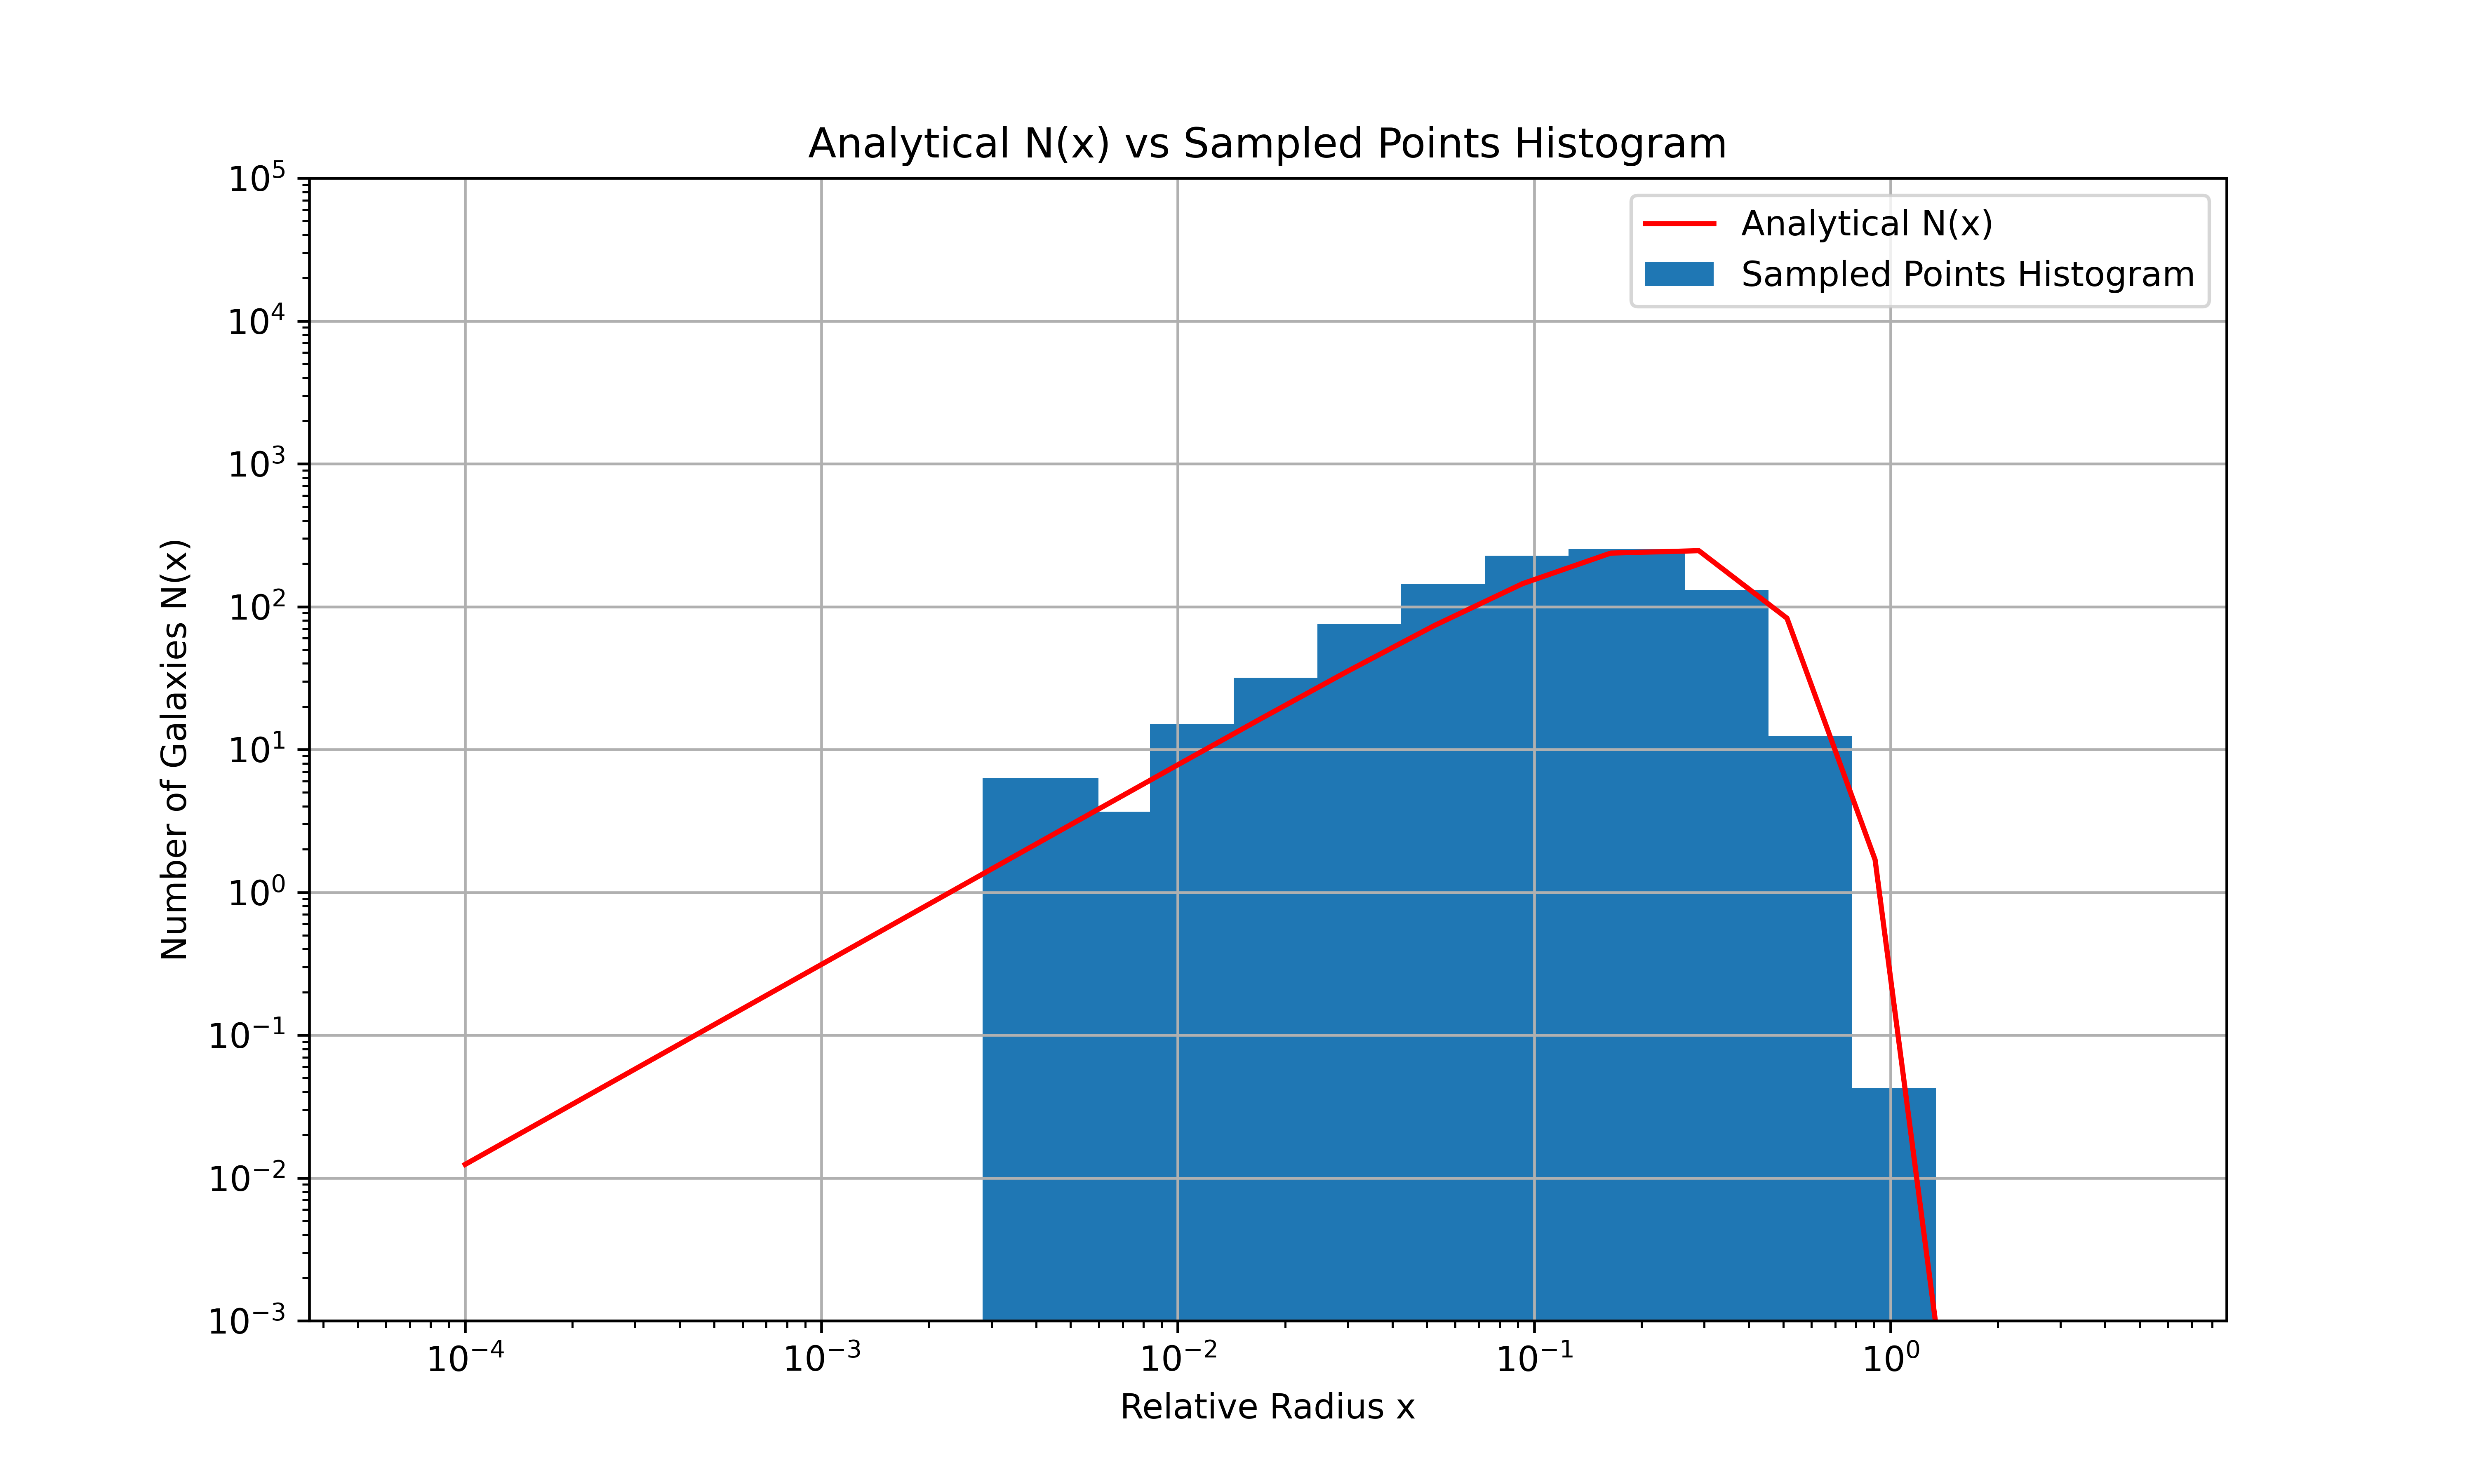
\includegraphics[width=0.9\linewidth]{./plots/my_solution_1b.png}
  \caption{Plot in logarithmic scale showing $N(x)$, function of the number of galaxies at given distance $x$, and the histogram of the 10000 sampled points. The sampled points match the analytical distribution.}
  \label{fig:n_vs_hist}
\end{figure}

For question (c), we select 100 random galaxies from the ones sampled in point (b), using Reservoir method. It is a sampling algorithm that chooses a random sample, without replacement, of $k$ items from a population of unknown size $n$ in a single pass over the items. The 100 drawn galaxies are ordered from smallest to largest radius. We do this as follow: \lstinputlisting[firstline=286,lastline=330]{satellite.py}
The number of galaxies within a radius $x$ are shown in Fig. \ref{fig:cum_galaxies}. The radii selected are starting from higher values because of the previous undersampling at lower values. The increasing trend makes sense as the number of galaxies within a given radius should increase as the radius increases.

\begin{figure}[h!]
  \centering
  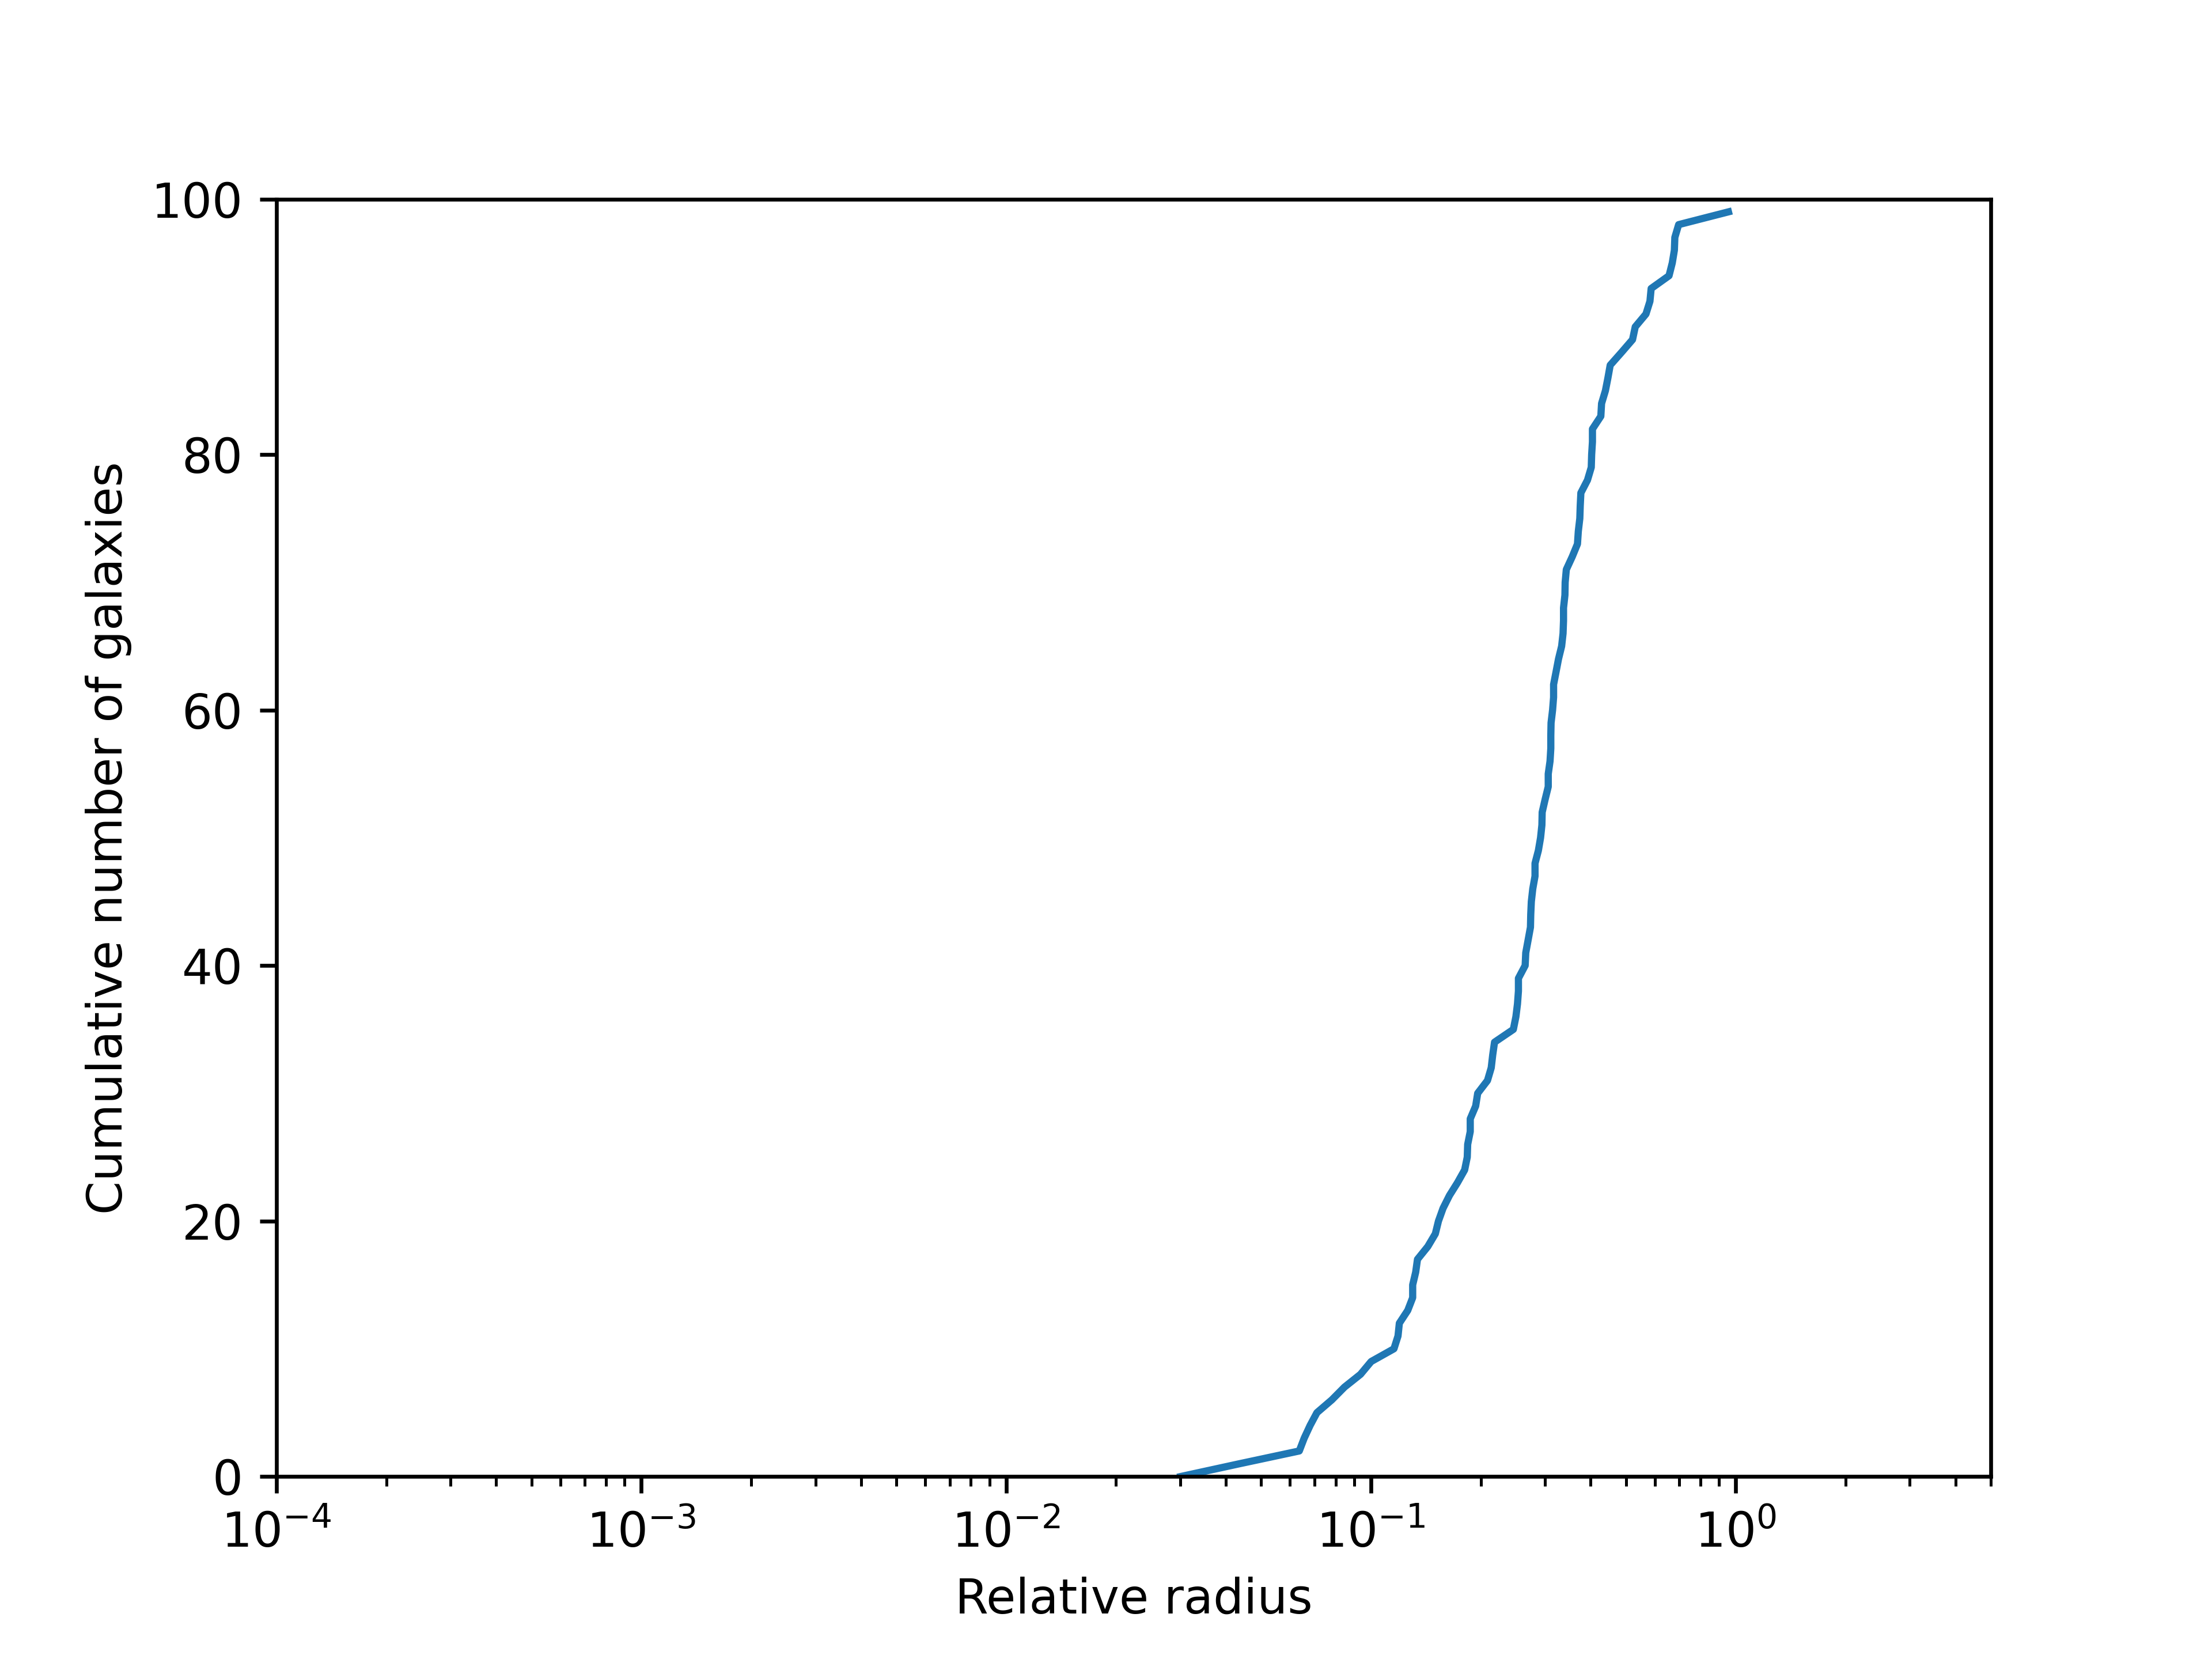
\includegraphics[width=0.9\linewidth]{./plots/my_solution_1c.png}
  \caption{Plot showing the cumulative number of galaxies randomly selected with respect to the relative radius $x$. The number of galaxies progressively increases with larger distances.}
  \label{fig:cum_galaxies}
\end{figure}

For question (d), we compute the derivative of the function $n(x)$ using both the Ridders' method and the analytical procedure. The code is below: \lstinputlisting[firstline=266,lastline=310]{satellite.py}
The obtained results can be seen in: \lstinputlisting{derivative.txt}


\section{Heating and cooling in HII regions}
The code relative to this exercise is in the script heating.py. The code relative to point (a) is the following: \lstinputlisting[firstline=8,lastline=68]{heating.py} The output of point (a) is in \lstinputlisting{2a.txt} 
For point (b), we have adopted again the bisection method, which guarantees convergence to a root of the function within a given interval, provided that the function is continuous and changes sign within that interval. It has a linear rate of convergence, which makes it slower with respect to other approaches, e.g. the secant method. We tried also this approach but the time taken for this specific problem was approximately the same and it experienced divergence from the expected root. The code follows the same structure as the one implemented in point (a), now taking into account the density variable $n_\text{e}$. The code is reported below: \lstinputlisting[firstline=70,lastline=135]{heating.py}
The output of (b) is in \lstinputlisting{2b.txt}
These results represent the equilibrium temperature of the ionized gas in HII regions. This quantity is determined by the balance between heating and cooling processes, which involve various physical phenomena such as free-free emission ($\Lambda_\text{FF}$), heating by cosmic rays ($\Gamma_\text{CR}$), and MHD waves ($\Gamma_{MHD}$).
\begin{itemize}
  \item For \textbf{low-density} gas ($n_\text{e} = 10^{-4} \, \text{cm}^{-3}$), the equilibrium temperature is extremely high ($1.60 \times 10^{14}$ K). This is because, at low densities, the cooling processes (like free-free emission which depends on the square of the density) are inefficient, and the gas remains hot.
  \item For \textbf{intermediate-density} gas ($n_\text{e} = 1 \, \text{cm}^{-3}$), the equilibrium temperature drops to $34243.13$ K. At these densities, the cooling processes become more efficient, and the gas can cool down to lower temperatures.
  \item For \textbf{high-density} gas ($n_\text{e} = 10^{4} \, \text{cm}^{-3}$), the equilibrium temperature is quite low ($29.12$ K). At high densities, the cooling processes are very efficient, and the gas can cool down to very low temperatures.
\end{itemize}


